\documentclass[11pt, a4paper]{scrartcl}
\usepackage{azzam}

\begin{document}

\section*{Mini Simulation 1 OSK SMP 2026: 6 Mei 2026}

\begin{enumerate}
    % 15. D
    \item Misalkan $ABCD$ adalah persegi panjang sedemikian sehingga $AB=3$ dan $BC=4$. Misalkan $M$ dan $N$ adalah pusat lingkaran yang tertulis di dalam segitiga $\triangle ABC$ dan $\triangle ADC$ masing-masing. Berapakah $MN^{2}$?
        \begin{center}
        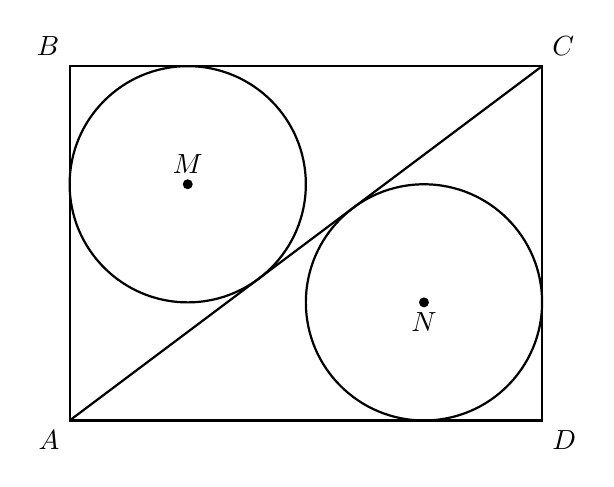
\begin{tikzpicture}[scale=1.5, thick]
        % Coordinates
        \coordinate (A) at (0,0);
        \coordinate (B) at (0,3);
        \coordinate (C) at (4,3);
        \coordinate (D) at (4,0);
        \coordinate (M) at (1,2);
        \coordinate (N) at (3,1);
    
        % Draw rectangle and diagonal
        \draw (A) -- (B) -- (C) -- (D) -- cycle;
        \draw (A) -- (C);
    
        % Draw inscribed circles
        \draw (M) circle (1);
        \draw (N) circle (1);
    
        % Draw centers and labels
        \fill (M) circle (1.2pt) node[above] {$M$};
        \fill (N) circle (1.2pt) node[below] {$N$};
    
        % Draw corner labels
        \node[below left] at (A) {$A$};
        \node[above left] at (B) {$B$};
        \node[above right] at (C) {$C$};
        \node[below right] at (D) {$D$};
    \end{tikzpicture}
    \end{center}
    \begin{itemize}
        \item[(A)] 2
        \item[(B)] 3
        \item[(C)] 4
        \item[(D)] 5
        \item[(E)] 6
    \end{itemize}

    % 16. E
    \item Sebuah belah ketupat memiliki tinggi 15 dan diagonal dengan rasio panjang 3:4. Berapakah panjang diagonal terpanjang dari belah ketupat tersebut?
    \begin{itemize}
        \item[(A)] 10
        \item[(B)] $\frac{25}{2}$
        \item[(C)] 15
        \item[(D)] 20
        \item[(E)] 25
    \end{itemize}

    % 18. C
    \item Definisikan barisan $\{a_{k}\}$ sedemikian sehingga $a_{k}=1!+2!+3!+\dots+k!$ untuk setiap bilangan bulat positif $k$. Untuk berapa banyak bilangan bulat positif $1\le n\le 2013$ sehingga kuantitas $a_{1}+a_{2}+a_{3}+\dots+a_{n}$ berakhiran dengan digit 3?
    \begin{itemize}
        \item[(A)] 100
        \item[(B)] 201
        \item[(C)] 202
        \item[(D)] 203
        \item[(E)] 403
    \end{itemize}

    % 19. C
    \item Untuk setiap bilangan bulat positif $n$, misalkan $a_{n}=\frac{n^{2}}{2n+1}$. Selanjutnya, misalkan $P$ dan $Q$ adalah bilangan riil sedemikian sehingga $P=a_{1}a_{2}\dots a_{2013}$ and $Q=(a_{1}+1)(a_{2}+1)\dots(a_{2013}+1)$. Berapakah jumlah digit-digit dari $\lfloor\frac{Q}{P}\rfloor$?
    \begin{itemize}
        \item[(A)] 27
        \item[(B)] 29
        \item[(C)] 31
        \item[(D)] 33
        \item[(E)] 35
    \end{itemize}

    % 20. A
    \item Salah satu adegan yang dihapus dari film Inception melibatkan sebuah persegi yang menggantung di udara pada sudut tertentu. Ellen mampu memperpanjang sisi-sisi persegi tersebut hingga menyentuh tanah pada titik-titik $P, A, G,$ and $E$ sesuai urutan tersebut. Pengukuran sederhana menunjukkan bahwa $PA=2$ and $GE=3$. Berapakah luas persegi tersebut?
    \begin{itemize}
        \item[(A)] $\frac{36}{13}$
        \item[(B)] 3
        \item[(C)] $\frac{48}{13}$
        \item[(D)] $\frac{23}{4}$
        \item[(E)] 4
    \end{itemize}

    % 21. D
    \item Pada $\triangle ABC$, $AB=13$, $AC=14$, and $BC=15$. Misalkan $M$ melambangkan titik tengah $\overline{AC}$. Titik $P$ diletakkan pada segmen garis $\overline{BM}$ sedemikian sehingga $\overline{AP}\perp\overline{PC}$. Misalkan $p, q,$ and $r$ adalah bilangan bulat positif dengan $p$ and $r$ relatif prima dan $q$ bebas kuadrat sedemikian sehingga luas $\triangle APC$ dapat ditulis dalam bentuk $\frac{p\sqrt{q}}{r}$. Berapakah $p+q+r$?
    \begin{itemize}
        \item[(A)] 221
        \item[(B)] 257
        \item[(C)] 302
        \item[(D)] 368
        \item[(E)] 391
    \end{itemize}

    % 22. A
    \item Lima timbangan berat, dilabeli A, B, C, D, dan E, diletakkan bersisian di atas meja. Richard ingin mendistribusikan delapan beban identik seberat 5 ons di antara kelima timbangan ini. Namun, jika berat gabungan pada salah satu timbangan melebihi 15 ons, timbangan tersebut akan rusak. Ada berapa banyak cara Richard dapat mendistribusikan beban tersebut sehingga tidak ada satu pun dari kelima timbangan yang rusak?
    \begin{itemize}
        \item[(A)] 155
        \item[(B)] 160
        \item[(C)] 165
        \item[(D)] 175
        \item[(E)] 190
    \end{itemize}

    % 23. E
    \item Sebuah bilangan bulat dikatakan "terpisah-dua" jika dapat dinyatakan sebagai hasil kali dua bilangan bulat positif yang berselisih dua. Demikian pula, sebuah bilangan bulat dikatakan "terpisah-sembilan" jika dapat dinyatakan sebagai hasil kali dua bilangan bulat positif yang berselisih 9. Berapakah jumlah dari semua bilangan bulat positif yang merupakan terpisah-dua sekaligus terpisah-sembilan?
    \begin{itemize}
        \item[(A)] 460
        \item[(B)] 424
        \item[(C)] 396
        \item[(D)] 375
        \item[(E)] 360
    \end{itemize}

    % 24. A
    \item Berapa banyak himpunan bagian $A$ dan $B$ yang saling lepas dari $\{1, 2, 3, 4, 5, 6, 7, 8\}$ sedemikian sehingga $|A|+|B|\in A$ dan $|A|-|B|\in B$?
    \begin{itemize}
        \item[(A)] 294
        \item[(B)] 316
        \item[(C)] 342
        \item[(D)] 363
        \item[(E)] 375
    \end{itemize}

    % 25. B
    \item Misalkan $P(x)=(x^{2}-x+1)(x^{4}-x^{2}+1)(x^{8}-x^{4}+1)\dots(x^{1024}-x^{512}+1)$. Ketika $P(x)$ dijabarkan, ada berapa banyak suku yang dikandungnya?
    \begin{itemize}
        \item[(A)] 1025
        \item[(B)] 1365
        \item[(C)] 1679
        \item[(D)] 1885
        \item[(E)] 2043
    \end{itemize}
\end{enumerate}

\end{document}